\documentclass[14pt, a4paper]{extreport}
\usepackage{extsizes}
\usepackage[a4paper, left=30mm, right=15mm, top=20mm, bottom=20mm]{geometry}
\usepackage[english, russian]{babel}
\usepackage{fontspec}
\defaultfontfeatures{Ligatures={TeX},Renderer=Basic}
\setmainfont[Ligatures={TeX,Historic}]{Times New Roman}
\usepackage{amsmath,amssymb}
\usepackage{graphicx}
\usepackage{setspace}
\graphicspath{{images/}}
\usepackage[hidelinks]{hyperref}
\usepackage{indentfirst}
\setlength{\parindent}{1.25cm}
\usepackage[explicit,compact]{titlesec}
\usepackage{titletoc}
\newcommand{\doublerule}[1][.4pt]{%
	\noindent
	\makebox[0pt][l]{\rule[.6ex]{\linewidth}{#1}}%
	\rule[.3ex]{\linewidth}{#1}
}

\addto\captionsrussian{%
	\renewcommand{\contentsname}%
	{\centering{СОДЕРЖАНИЕ}}%
}

\usepackage{caption}
\DeclareCaptionLabelSeparator{dash}{ -- }
\DeclareCaptionLabelFormat{figure}{Рисунок #2}
\captionsetup[table]{
	labelsep=dash,
	singlelinecheck=false,
}
\captionsetup[figure]{
	labelsep=dash,
	labelformat=figure,
}

\usepackage{floatrow}
\floatsetup[table]{style=plaintop}
\floatsetup[equation]{style=plain}

\usepackage{chngcntr}
\counterwithout{figure}{chapter}
\counterwithout{equation}{chapter}
\counterwithout{table}{chapter}

\usepackage{cleveref}
\crefformat{table}{смотри табл.#2#1#3}
\Crefformat{table}{Смотри табл.#2#1#3}

\crefformat{figure}{рис.~#2#1#3}
\Crefformat{figure}{Рис.~#2#1#3}
\crefmultiformat{figure}{рис.~#2#1#3}{,~#2#1#3}{,~#2#1#3}{,~#2#1#3}

\crefformat{equation}{#1}

\begin{document}
\begin{titlepage}
	\begin{center}
		\vspace*{0.5mm}
		\setstretch{1.1}

		
\includegraphics[width=0.18\textwidth]{logo}\\
		\footnotesize
		МИНИСТЕРСТВО НАУКИ И ВЫСШЕГО ОБРАЗОВАНИЯ РОССИЙСКОЙ ФЕДЕРАЦИИ\\
		\small
		Федеральное государственное бюджетное образовательное учреждение высшего образования\\
		\textbf{«МИРЭА - Российский технологический университет»}
		\vspace{0.5cm}

		\large \textbf{РТУ МИРЭА} \normalsize

		\doublerule[1pt]\\
		\vspace{0.4cm}

		Институт искусственного интеллекта\\
		Кафедра общей информатики
		\vspace{1.5cm}

		\textbf{ОТЧЕТ}\\
		\textbf{ПО ПРАКТИЧЕСКОЙ РАБОТЕ № 5}\\
		\textbf{построение комбинационных схем, реализующих СДНФ и СКНФ заданной логической функции от 4-х переменных}\\
		\textbf{по дисциплине}\\
		«ИНФОРМАТИКА»
		\vspace{1.5cm}

		\small
		Выполнил студент группы ИМБО-01-22 \hfill Скирдин Никита Сергеевич
		\vspace{1cm}

		Принял \hfill Павлова Екатерина Сергеевна\\
		ассистент \hfill
		\vspace{1.5cm}

		\footnotesize
		\hspace{0.5cm} Практическая \hfill «\_\_»\_\_\_\_\_\_2022 г. \hfill Подпись студента\\
		\hspace{0.5cm} работа выполнена \hfill
		\vspace{0.5cm}

		\hspace{2cm} «Зачтено» \hfill «\_\_»\_\_\_\_\_\_2022 г. \hfill Подпись преподавателя
		\vfill

		\small
		Москва 2022
	\end{center}
	\thispagestyle{empty}
\end{titlepage}

\setstretch{1.5}
\setcounter{page}{2}

\titlecontents{chapter}[0em]
	{\vskip 0.5ex}%
	{\thecontentslabel \space \uppercase}% numbered sections formatting
	{}% unnumbered sections formatting
	{\hfill \thecontentspage}%

\titlecontents{section}[1.25cm]
	{\vskip 0.5ex}%
	{\thecontentslabel \space}
	{}
	{\hfill \thecontentspage}

\titleformat{\chapter}[block]
	{\bfseries\normalsize}{}{0pt}{\uppercase{#1}}

\titleformat{\section}[block]
	{\bfseries\normalsize}{}{0pt}{#1}

\titlespacing*{\chapter}{0pt}{-10.5mm}{0pt}

\tableofcontents

\titleformat{\chapter}[display]
	{\centering\bfseries\normalsize}{}{0pt}{\thechapter \space \uppercase{#1}}

\titleformat{\section}[block]
	{\hspace{\parindent}\bfseries\normalsize}{}{0pt}{\thesection \space #1}

\titlespacing*{\chapter}{0pt}{-19.5mm}{0pt}

\chapter{Постановка задачи}
Логическая функция от четырех переменных задана в 16-теричной векторной форме. Восстановить таблицу истинности. Записать формулы СДНФ и СКНФ. Построить комбинационные схемы СДНФ и СКНФ в лабораторном комплексе, используя общий логический базис. Протестировать работу схем и убедиться в их правильности. Подготовить отчет о проделанной  работе и защитить ее.

\section{Персональный вариант}
Логическая функция от четырех переменных, заданная в 16-теричной форме: F9AA$_{16}$

\chapter{Проектирование и реализация}
\section{Предварительная подготовка данных}
Преобразуем заданную логическую функцию в двоичную запись: 1111 1001 1010 1010$_2$ - получили столбец значений логической функции, который необходим для восстановления полной таблицы истинности (\cref{tab:1}).

\begin{table}[!htbp]
	\caption{Таблица истинности заданной функции}
	\label{tab:1}
	\begin{tabular}{|c|c|c|c|c|}
		\hline
		a & b & c & d & F \\
		\hline
		0 & 0 & 0 & 0 & 1 \\
		\hline
		0 & 0 & 0 & 1 & 1 \\
		\hline
		0 & 0 & 1 & 0 & 1 \\
		\hline
		0 & 0 & 1 & 1 & 1 \\
		\hline
		0 & 1 & 0 & 0 & 1 \\
		\hline
		0 & 1 & 0 & 1 & 0 \\
		\hline
		0 & 1 & 1 & 0 & 0 \\
		\hline
		0 & 1 & 1 & 1 & 1 \\
		\hline
		1 & 0 & 0 & 0 & 1 \\
		\hline
		1 & 0 & 0 & 1 & 0 \\
		\hline
		1 & 0 & 1 & 0 & 1 \\
		\hline
		1 & 0 & 1 & 1 & 0 \\
		\hline
		1 & 1 & 0 & 0 & 1 \\
		\hline
		1 & 1 & 0 & 1 & 0 \\
		\hline
		1 & 1 & 1 & 0 & 1 \\
		\hline
		1 & 1 & 1 & 1 & 0 \\
		\hline
	\end{tabular}
\end{table}

\section{Вывод формулы для СДНФ}
Запишем формулу СДНФ, для чего рассмотрим наборы значений переменных, на которых функция равна единице (\cref{tab:2}). Для каждого набора переменные, равные нулю, берем с отрицанием, а переменные, равные единице, без отрицания. В результате получим множество совершенных конъюнкций, объединив которые через дизъюнкцию, образуем формулу СДНФ (\cref{equ:1}).

\begin{table}[!htbp]
	\caption{Таблица СДНФ}
	\label{tab:2}
	\begin{tabular}{|c|c|c|c|c|}
		\hline
		a & b & c & d & F \\
		\hline
		0 & 0 & 0 & 0 & 1 \\
		\hline
		0 & 0 & 0 & 1 & 1 \\
		\hline
		0 & 0 & 1 & 0 & 1 \\
		\hline
		0 & 0 & 1 & 1 & 1 \\
		\hline
		0 & 1 & 0 & 0 & 1 \\
		\hline
		0 & 1 & 1 & 1 & 1 \\
		\hline
		1 & 0 & 0 & 0 & 1 \\
		\hline
		1 & 0 & 1 & 0 & 1 \\
		\hline
		1 & 1 & 0 & 0 & 1 \\
		\hline
		1 & 1 & 1 & 0 & 1 \\
		\hline
	\end{tabular}
\end{table}

\begin{align}
	\label{equ:1}
	F_\textup{СДНФ} = %
		  \bar{a} \cdot \bar{b} \cdot \bar{c} \cdot \bar{d}
		+ \bar{a} \cdot \bar{b} \cdot \bar{c} \cdot d
		+ \bar{a} \cdot \bar{b} \cdot c \cdot \bar{d}
		+ \bar{a} \cdot \bar{b} \cdot c \cdot d
		+ \bar{a} \cdot b \cdot \bar{c} \cdot \bar{d} + \\
		+ \bar{a} \cdot b \cdot c \cdot d
		+ a \cdot \bar{b} \cdot \bar{c} \cdot \bar{d}
		+ a \cdot \bar{b} \cdot c \cdot \bar{d}
		+ a \cdot b \cdot \bar{c} \cdot \bar{d}
		+ a \cdot b \cdot c \cdot \bar{d} \notag
\end{align}

\section{Вывод формулы для СКНФ}
Запишем формулу СКНФ, для чего рассмотрим наборы значений переменных, на которых функция равна нулю (\cref{tab:3}). Для каждого набора переменные, равные единице, надо взять с отрицанием, а переменные, равные нулю, без отрицания. В результате мы получим множество совершенных дизъюнкций, объединив которые через конъюнкцию образуем формулу СКНФ (\cref{equ:2}).

\begin{table}[!htbp]
	\caption{Таблица СКНФ}
	\label{tab:3}
	\begin{tabular}{|c|c|c|c|c|}
		\hline
		a & b & c & d & F \\
		\hline
		0 & 1 & 0 & 1 & 0 \\
		\hline
		0 & 1 & 1 & 0 & 0 \\
		\hline
		1 & 0 & 0 & 1 & 0 \\
		\hline
		1 & 0 & 1 & 1 & 0 \\
		\hline
		1 & 1 & 0 & 1 & 0 \\
		\hline
		1 & 1 & 1 & 1 & 0 \\
		\hline
	\end{tabular}
\end{table}

\begin{align}
	\label{equ:2}
	F_\textup{СКНФ} = %
			  (a + \bar{b} + c + \bar{d})
		\cdot (a + \bar{b} + \bar{c} + d)
		\cdot (\bar{a} + b + c + \bar{d}) \cdot \\
		\cdot (\bar{a} + b + \bar{c} + \bar{d})
		\cdot (\bar{a} + \bar{b} + c + \bar{d})
		\cdot (\bar{a} + \bar{b} + \bar{c} + \bar{d}) \notag
\end{align}

\section{Построение схем в лабораторном комплексе}
Построим в лабораторном комплексе комбинационные схемы, реализующие СДНФ и СКНФ рассматриваемой функции в общем логическом базисе, протестируем их работу и убедимся в их правильности (\cref{fig:1,fig:2}).

\begin{figure}[htbp]
	\centering
	\caption{Тестирование схемы СДНФ}
	\label{fig:1}
	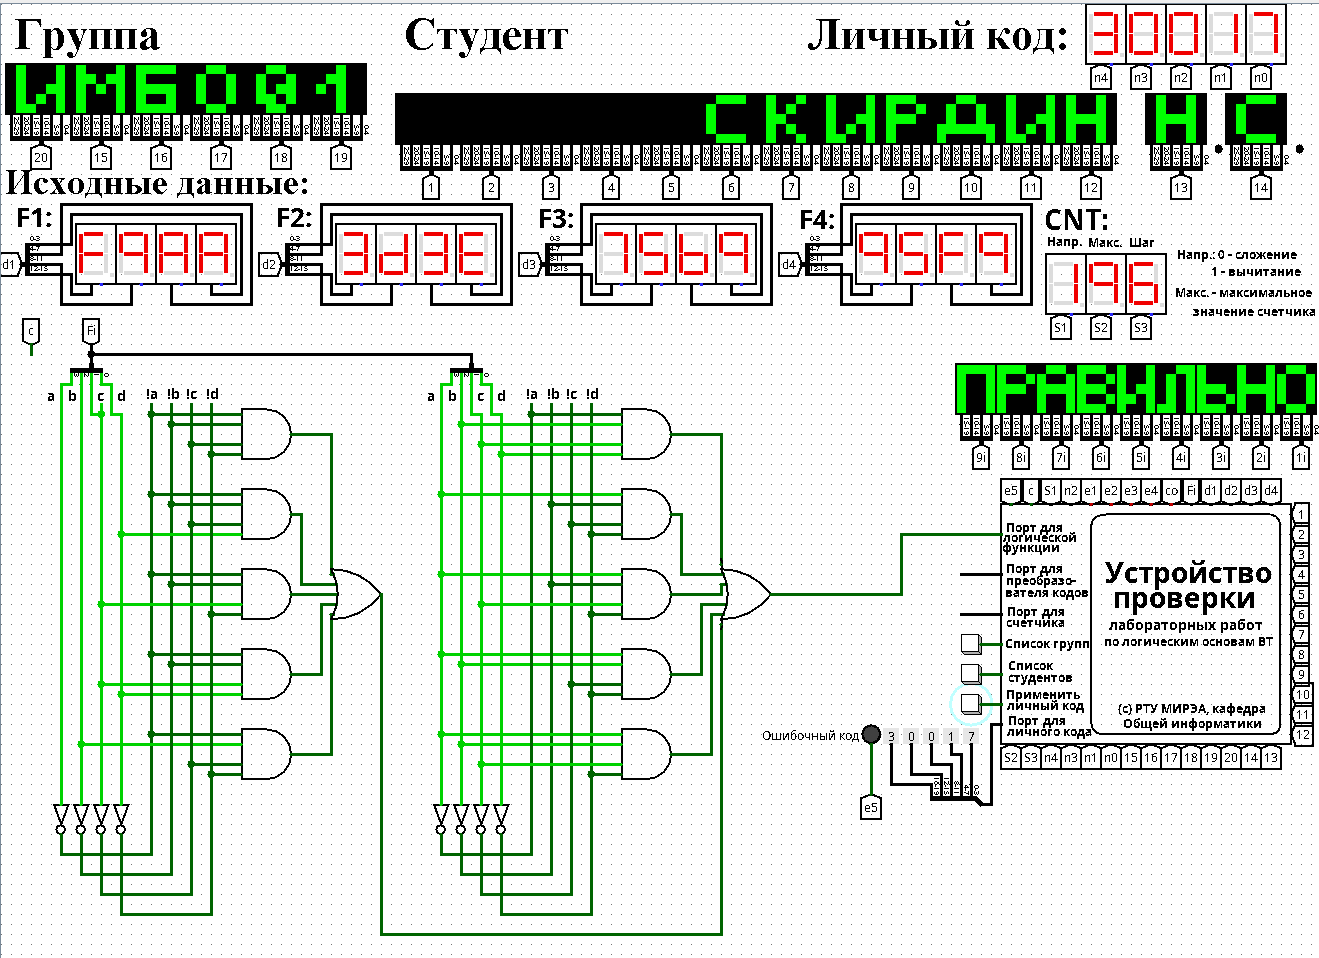
\includegraphics[width=\textwidth]{sdnf}\\
\end{figure}

\begin{figure}[p]
	\centering
	\caption{Тестирование схемы СКНФ}
	\label{fig:2}
	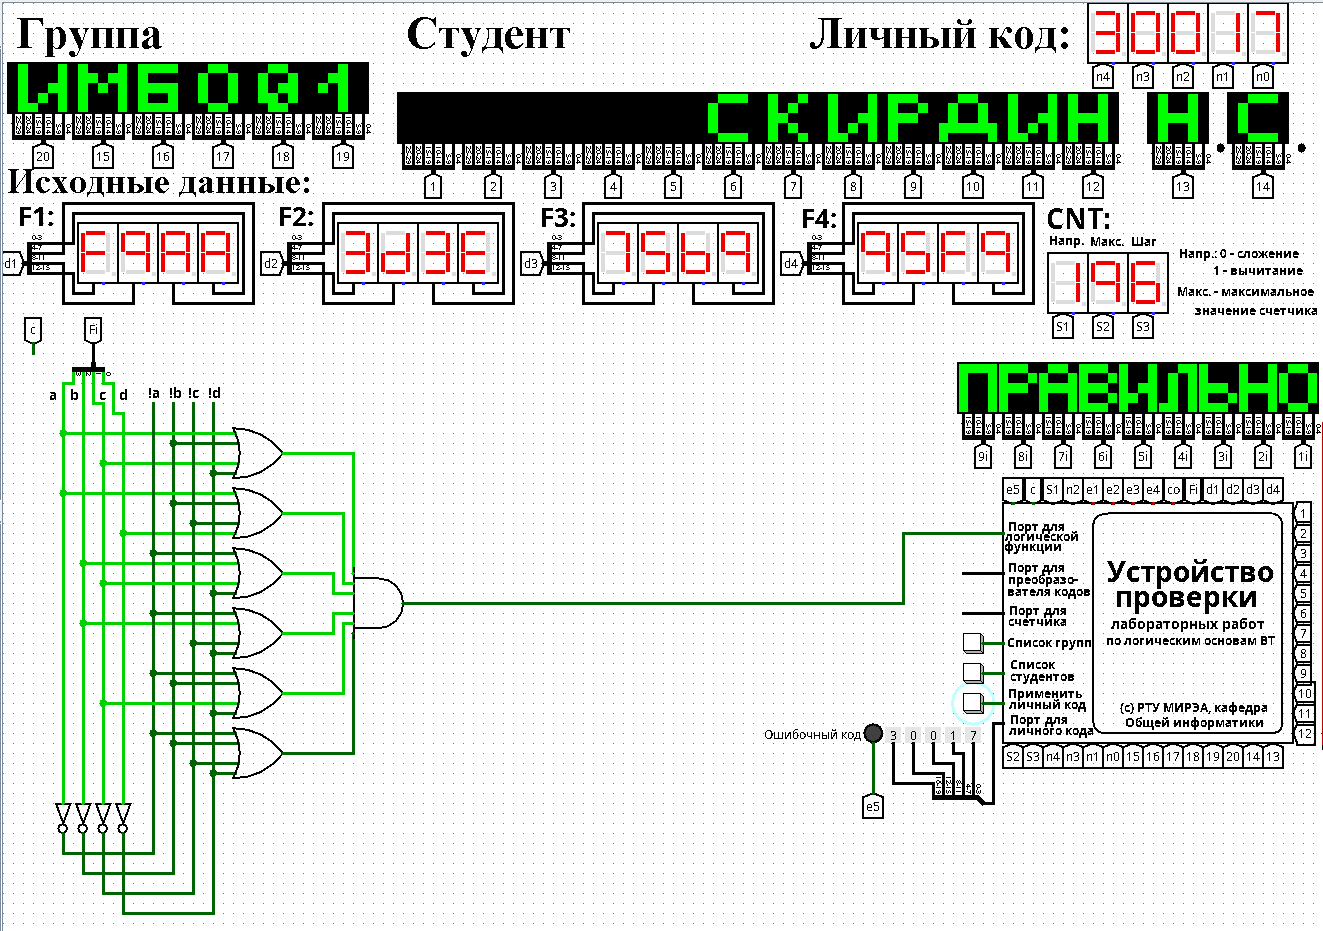
\includegraphics[width=\textwidth]{sknf}\\
\end{figure}

\makeatletter
\setlength{\@fptop}{0pt}
\makeatother

\chapter{Выводы}
Восстановил таблицу истинности заданной логической функции от четырех переменных. Записал для нее формулы СДНФ и СКНФ. Построил комбинационные схемы СДНФ и СКНФ в лабораторном комплексе, используя общий логический базис. Протестировал работу схем и убедился в их правильности.

\chapter{Информационный источник}
\textbf{Смирнов, С. С.} Информатика : Методические указания по выполнению практических работ / С. С. Смирнов, Д. А. Карпов. -- Москва : МИРЭА -- Российский технологический университет, 2020. -- 102 с.

\end{document}
